This chapter provides a quick hands-on introduction to using Haizea in simulation mode. Even if you intend to use Haizea in combination with another system, such as OpenNebula, you may still find this guide useful to familiarise yourself with the Haizea configuration file and command-line interface. This chapter assumes that Haizea is installed on your system. If you have arrived at this chapter directly, you may want to read Chapter~\ref{chap:whatis} (``What is Haizea?'') first, although you should still be able to follow the instructions in this chapter without reading Chapter~\ref{chap:whatis} first.

\section{The \texttt{haizea} command}

The main command in the Haizea system is, unsurprisingly, the \texttt{haizea} command. Running this command starts up the Haizea lease manager, which is then ready to receive and schedule lease requests. As described in Chapter~\ref{chap:whatis}, Haizea can run in one of three modes: unattended simulated mode, interactive simulated mode, and OpenNebula mode. In this chapter we will focus on the simulation modes, starting with the ``unattended'' variety. Both simulation modes, and the OpenNebula mode, will be described in more detail in the next chapters.

When running Haizea in unattended simulation mode, the inputs to Haizea are going to be the following:

\begin{description}
 \item [The Haizea configuration file:] A text file containing all the options
 \item [A request \emph{tracefile}:] A text file containing a list of lease requests. Since we are using ``simulated time'', we won't be able to use Haizea interactively (we will be able to do this when we switch to the ``real time'' mode later in the chapter). Instead, we need to provide all the lease requests beforehand.
\end{description}

Based on the configuration file and the lease requests, the simulator produces a schedule for those leases, which you will be able to follow through logging messages printed by Haizea. At the end of the simulation, Haizea also saves a fair amount of raw data and statistics to disk which can be used to produce reports and graphs (a module to do this for you is in the works). This particular mode, with simulated time, is particularly useful when you want to take a list of request (potentially spanning weeks or months) to see what happens when you tweak the scheduling options (without having to wait weeks or months for the result).

So, let's start by writing a configuration file specifying the simulation options (e.g., the characteristics of the simulated cluster) and the scheduling options.

\section{The configuration file}

A sample configuration file is provided with Haizea and is located in \texttt{/usr/share/haizea/etc/sample\_trace.conf} (or \texttt{\$HOME/share/haizea/etc/sample\_trace.conf} if you installed Haizea in your home directory). For this guide, you may want to make a copy of this file and use that instead (so you can preserve the original sample file). If you look at the contents of the file, you will see that it also includes documentation on every option (if you find the documentation gets in the way, there is also a \texttt{sample\_trace\_barebones.conf} file that has the same options, but without any documentation). For now, take a look at the following three options:

\begin{wideshellverbatim}
[simulation]
starttime: 2006-11-25 13:00:00
resources: 4  CPU:100 Memory:1024
\end{wideshellverbatim}

These options are used to describe the characteristics of our simulated cluster. In particular, we're using a 4-node cluster, each node with 1 CPU, 1024 MB of memory. In this document, we will represent this cluster over time like this:

\begin{center}
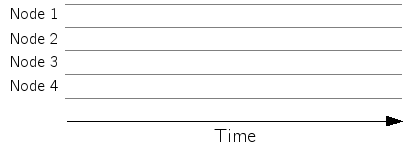
\includegraphics{images/quickstart_leasegraph1.png}
\end{center}

For example, the following figure shows a lease scheduled on Node 1 from 13:00 to 14:00:

\begin{center}
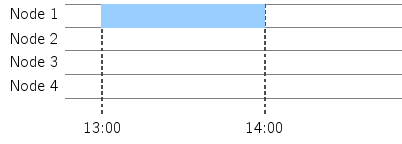
\includegraphics{images/quickstart_leasegraph2.png}
\end{center}

The \texttt{starttime} option is used to specify the time at which the simulated clock should start. As you will see, the configuration file has an abundance of other options. We will cover some of them in this chapter, but a more complete reference can be found in Appendix~\ref{app:conffile}.

\section{The tracefile}

As mentioned earlier, the simulator will read trace requests from a tracefile. The location of this tracefile is specified in the configuration file, in the \texttt{[tracefile]} section:

\begin{wideshellverbatim}
[tracefile]
tracefile: /usr/share/haizea/traces/sample.lwf 
\end{wideshellverbatim}

The default value is a sample tracefile included with Haizea. If you copy the file to a different location, make sure to update the \texttt{tracefile} option accordingly. The format of this file is LWF (Lease Workload Format), an XML format which is particular to Haizea. For now, don't worry about parsing the trace format in detail; it is fairly human-readable and you can also find details on the LWF format in Appendix~\ref{app:lwf}.

\begin{wideshellverbatim}
<lease-workload name="sample">
	<description>
	A simple trace where an AR lease preempts a 
	best-effort lease that is already running. 
	</description>

	<lease-requests>
	
	<!-- The lease requests are initially commented out -->
	
	<!-- First lease request -->
	<!--
	...
	-->

	<!-- Second lease request -->
	<!--
	...
	-->
	
	</lease-requests>
</lease-workload>
\end{wideshellverbatim}

As you can see, there are two lease requests in the file, but they are initially commented out. We will take a closer look at each of these requests next.

\section{Running the simulator}

Now that we have a configuration file and a tracefile, we can run the simulator. You can run Haizea with the sample configuration file like this:

\begin{shellverbatim}
haizea -c /usr/share/haizea/etc/sample_trace.conf 
\end{shellverbatim}

Which results in the following output:

\begin{wideshellverbatim}
[2006-11-25 13:00:00.00] RM      Starting resource manager
[2006-11-25 13:00:00.00] TFILE   Loading tracefile /usr/share/haizea/traces/sample.lwf
[2006-11-25 13:00:00.00] TFILE   Loaded workload with 0 requests ()
[2006-11-25 13:00:00.00] CLOCK   Starting simulated clock
[2006-11-25 13:00:00.00] CLOCK   Simulated clock has stopped
[2006-11-25 13:00:00.00] RM      Stopping resource manager gracefully...
[2006-11-25 13:00:00.00] RM      --- Haizea status summary ---
[2006-11-25 13:00:00.00] RM      Number of leases (not including completed): 0
[2006-11-25 13:00:00.00] RM      Completed leases: 0
[2006-11-25 13:00:00.00] RM      Completed best-effort leases: 0
[2006-11-25 13:00:00.00] RM      Queue size: 0
[2006-11-25 13:00:00.00] RM      Accepted AR leases: 0
[2006-11-25 13:00:00.00] RM      Rejected AR leases: 0
[2006-11-25 13:00:00.00] RM      Accepted IM leases: 0
[2006-11-25 13:00:00.00] RM      Rejected IM leases: 0
[2006-11-25 13:00:00.00] RM      ---- End summary ----
\end{wideshellverbatim}

Now that you've seen the tracefile, you can see why the simulator starts up and immediately stops: all the lease requests in the tracefile are commented out, and there's nothing to schedule. Go ahead and uncomment the first lease request, which looks like this:

\begin{wideshellverbatim}
<lease-request arrival="00:00:00">
<lease preemptible="true">
	<nodes>
		<node-set numnodes="1">
			<res type="CPU" amount="100"/>
			<res type="Memory" amount="1024"/>
		</node-set>
	</nodes>	
	<start></start>
	<duration time="01:00:00"/>
	<software>
		<disk-image id="foobar.img" size="1024"/>
	</software>
</lease>
</lease-request>
\end{wideshellverbatim}

This is a request for a best-effort lease (notice how the starting time is left empty, meaning it's up to Haizea to determine the start time), requested at time 00:00:00 (right at the start of the simulation), requiring 1 hour, and only one node. Now run Haizea again. You should now see the following:

\begin{wideshellverbatim}
[2006-11-25 13:00:00.00] RM      Starting resource manager
[2006-11-25 13:00:00.00] TFILE   Loading tracefile /usr/share/haizea/traces/sample.lwf
[2006-11-25 13:00:00.00] TFILE   Loaded workload with 1 requests (1 Best-effort)
[2006-11-25 13:00:00.00] CLOCK   Starting simulated clock
[2006-11-25 13:00:00.00] LSCHED  Lease #1 has been requested.
[2006-11-25 13:00:00.00] LSCHED  Lease #1 has been marked as pending.
[2006-11-25 13:00:00.00] LSCHED  Queued best-effort lease request #1, 1 nodes for 01:00:00.00.
[2006-11-25 13:00:00.00] LSCHED  Next request in the queue is lease 1. Attempting to schedule...
[2006-11-25 13:00:00.00] VMSCHED Lease #1 has been scheduled on nodes [1] 
                                 from 2006-11-25 13:00:00.00 
                                   to 2006-11-25 14:00:00.00
[2006-11-25 13:00:00.00] VMSCHED Started VMs for lease 1 on nodes [1]
[2006-11-25 14:00:00.00] VMSCHED Stopped VMs for lease 1 on nodes [1]
[2006-11-25 14:00:00.00] VMSCHED Lease 1's VMs have shutdown.
[2006-11-25 14:00:00.00] CLOCK   Simulated clock has stopped
[2006-11-25 14:00:00.00] RM      Stopping resource manager gracefully...
[2006-11-25 14:00:00.00] RM      --- Haizea status summary ---
[2006-11-25 14:00:00.00] RM      Number of leases (not including completed): 0
[2006-11-25 14:00:00.00] RM      Completed leases: 1
[2006-11-25 14:00:00.00] RM      Completed best-effort leases: 1
[2006-11-25 14:00:00.00] RM      Queue size: 0
[2006-11-25 14:00:00.00] RM      Accepted AR leases: 0
[2006-11-25 14:00:00.00] RM      Rejected AR leases: 0
[2006-11-25 14:00:00.00] RM      Accepted IM leases: 0
[2006-11-25 14:00:00.00] RM      Rejected IM leases: 0
[2006-11-25 14:00:00.00] RM      ---- End summary ----
\end{wideshellverbatim}

The above corresponds to the following schedule:

\begin{center}
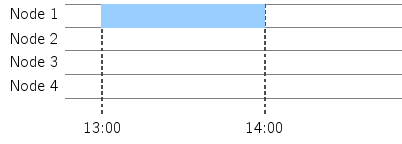
\includegraphics{images/quickstart_leasegraph2.png}
\end{center}

A best-effort request is received at 13:00 and, since the cluster is empty, it is scheduled immediately. Notice how the VMs for the lease start at 13:00 and stop at 14:00. For now, we're assuming that the disk images are predeployed on the physical nodes (we will modify this option in the next section).

Now go ahead and uncomment the second lease request, which looks like this:

\begin{wideshellverbatim}
<lease-request arrival="00:15:00">
<lease preemptible="false">
	<nodes>
		<node-set numnodes="4">
			<res type="CPU" amount="100"/>
			<res type="Memory" amount="1024"/>
		</node-set>
	</nodes>
	<start>
		<exact time="00:30:00"/>
	</start>
	<duration time="00:30:00"/>
	<software>
		<disk-image id="foobar.img" size="1024"/>
	</software>
</lease>
</lease-request>
\end{wideshellverbatim}

This is a request for an advance reservation lease (notice how there is an exact starting time specified), requesting all four nodes for 30 minutes. So, what would happen if we also added this AR lease? Since it requires all the cluster resources from 13:30 to 14:00, the best-effort lease will be unable to run in that time interval. Since the leases are implemented as VMs, Haizea will still schedule the best-effort lease to start at 13:00, but will suspend it before the AR lease starts, and will resume it once the AR lease has finished. In effect, we want the schedule to look like this:

\begin{center}
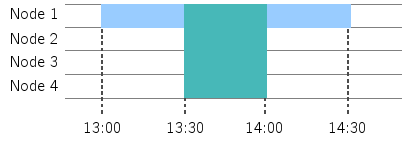
\includegraphics{images/quickstart_leasegraph3.png}
\end{center}

Uncomment the AR lease request, and run Haizea again. You should now see the following:

\begin{wideshellverbatim}
[2006-11-25 13:00:00.00] RM      Starting resource manager
[2006-11-25 13:00:00.00] TFILE   Loading tracefile /usr/share/haizea/traces/sample.lwf
[2006-11-25 13:00:00.00] TFILE   Loaded workload with 2 requests (1 Best-effort + 1 AR)
[2006-11-25 13:00:00.00] CLOCK   Starting simulated clock
[2006-11-25 13:00:00.00] LSCHED  Lease #1 has been requested.
[2006-11-25 13:00:00.00] LSCHED  Lease #1 has been marked as pending.
[2006-11-25 13:00:00.00] LSCHED  Queued best-effort lease request #1, 1 nodes for 01:00:00.00.
[2006-11-25 13:00:00.00] LSCHED  Next request in the queue is lease 1. Attempting to schedule...
[2006-11-25 13:00:00.00] VMSCHED Lease #1 has been scheduled on nodes [1] 
                                 from 2006-11-25 13:00:00.00 
                                   to 2006-11-25 14:00:00.00
[2006-11-25 13:00:00.00] VMSCHED Started VMs for lease 1 on nodes [1]

[2006-11-25 13:15:00.00] LSCHED  Lease #2 has been requested.
[2006-11-25 13:15:00.00] LSCHED  Lease #2 has been marked as pending.
[2006-11-25 13:15:00.00] LSCHED  Scheduling AR lease #2, 4 nodes
                                 from 2006-11-25 13:30:00.00 
                                   to 2006-11-25 14:00:00.00.
[2006-11-25 13:15:00.00] LSCHED  Must preempt leases [1] to make room for lease #2
[2006-11-25 13:15:00.00] LSCHED  Preempting lease #1...
[2006-11-25 13:15:00.00] LSCHED  ... lease #1 will be suspended 
                                     at 2006-11-25 13:30:00.00.
[2006-11-25 13:15:00.00] LSCHED  AR lease #2 has been scheduled.

[2006-11-25 13:29:28.00] VMSCHED Stopped VMs for lease 1 on nodes [1]
[2006-11-25 13:29:28.00] VMSCHED Suspending lease 1...

[2006-11-25 13:30:00.00] VMSCHED Lease 1 suspended.
[2006-11-25 13:30:00.00] VMSCHED Started VMs for lease 2 on nodes [2, 3, 4, 1]
[2006-11-25 13:30:00.00] LSCHED  Next request in the queue is lease 1. Attempting to schedule...
[2006-11-25 13:30:00.00] VMSCHED Lease #1 has been scheduled on nodes [1]
                                 from 2006-11-25 14:00:00.00 (resuming) 
                                   to 2006-11-25 14:31:04.00

[2006-11-25 14:00:00.00] VMSCHED Stopped VMs for lease 2 on nodes [2, 3, 4, 1]
[2006-11-25 14:00:00.00] VMSCHED Resuming lease 1...
[2006-11-25 14:00:00.00] VMSCHED Lease 2's VMs have shutdown.

[2006-11-25 14:00:32.00] VMSCHED Resumed lease 1
[2006-11-25 14:00:32.00] VMSCHED Started VMs for lease 1 on nodes [1]

[2006-11-25 14:31:04.00] VMSCHED Stopped VMs for lease 1 on nodes [1]
[2006-11-25 14:31:04.00] VMSCHED Lease 1's VMs have shutdown.
[2006-11-25 14:31:04.00] CLOCK   Simulated clock has stopped
[2006-11-25 14:31:04.00] RM      Stopping resource manager gracefully...
\end{wideshellverbatim}

Notice how the above corresponds to the previous figure. In particular, notice the following:

\begin{itemize}
 \item  When the AR lease request is received, Haizea looks at the schedule and determines that the only way to schedule the AR lease is to preempt the best-effort lease. However, instead of cancelling that lease, it will just reschedule it so it is suspended right before the AR lease start. Note that Haizea will always try to minimise the number of preemption (in this case, we're forcing the situation for demonstration purposes) by assigning the AR lease to resources that are available without preempting other leases.
 \item Shortly before the AR lease starts, the best-effort lease is suspended (the time required to do this is estimated by Haizea based on an option in the configuration file). When the AR lease ends at 14:00, Haizea begins resuming the suspended best-effort lease.
\end{itemize}

\section{The scheduling options}

Haizea has several scheduling options that control how Haizea selects resources and schedules leases. For example, the above example assumed that leases can be suspended (which they generally always can be when running as virtual machines). What would happen if this were not possible? You can modify the suspension option in the \texttt{[scheduling]} section to find out:

\begin{wideshellverbatim}
[scheduling]
...

suspension: none

...
\end{wideshellverbatim}

Rerun Haizea. Now, when the AR lease arrives at 13:15, the scheduler will realise it has to preempt the best-effort lease to make room for the AR lease, but will no longer be able to suspend it. The only option is to cancel the best-effort lease and resubmit it to the queue:

\begin{wideshellverbatim}
[2006-11-25 13:15:00.00] LSCHED  Preempting lease #1...
[2006-11-25 13:15:00.00] LSCHED  ... lease #1 has been cancelled and requeued
\end{wideshellverbatim}

Now, the best-effort lease can only be scheduled after the AR lease, at 14:00:

\begin{wideshellverbatim}
[2006-11-25 13:15:00.00] VMSCHED Lease #1 has been scheduled on nodes [1] 
                                 from 2006-11-25 14:00:00.00 
                                   to 2006-11-25 15:00:00.00
\end{wideshellverbatim}

So, the schedule would end up looking like this:

\begin{center}
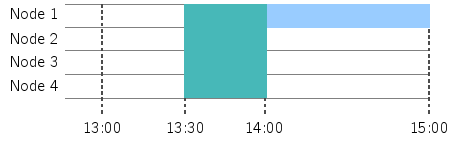
\includegraphics{images/quickstart_leasegraph4.png}
\end{center}

Notice how, although suspending a lease is a disruptive activity which can delay the completion time of a best-effort request, it is still much better than completely cancelling a request and waiting for enough resources to accommodate the entire (uninterrupted) duration of the lease.

Another scheduling option you can modify is whether Haizea should transfer the VM's disk image from an image repository before the lease can start. You can do this by modifying the \texttt{lease-deployment} option:

\begin{wideshellverbatim}
[general]
...
lease-preparation: imagetransfer
...
\end{wideshellverbatim}

If you look at the bottom of the sample configuration file, you will find a section called \texttt{[deploy-imagetransfer]} with all the image transfer options.

Rerun Haizea again. You should get a schedule similar to the previous one, but with some extra messages indicating that image transfers are taking place:

\begin{wideshellverbatim}
[2006-11-25 13:00:00.00] DEPLOY  Starting image transfer for lease 1
[2006-11-25 13:01:22.00] DEPLOY  Completed image transfer for lease 1
\end{wideshellverbatim}

As you can see, the best-effort lease can no longer start right at 13:00, since an image transfer has to take place before the starting time. The same is true of the AR lease, but notice how Haizea schedules the image transfer in such a way that the AR lease can still start at 13:30 as planned (instead of delaying the starting time until 13:31:22).

There are several other options you can modify in the \texttt{[scheduling]} section, such as what backfilling algorithm to use, whether to allow lease migration or not, etc. These options are described in the following chapters, and in Appendix~\ref{app:conffile}.

\section{Interactive simulations} 

Up to this point, Haizea has been scheduling leases in ``simulated time''. This meant that we provided Haizea with a lease workload beforehand, ran it, and got the results of scheduling that workload much earlier than it would have actually taken to run the leases (e.g., if we requested a 30 minute lease, we didn't have to wait 30 minutes for the lease to complete; Haizea just skipped from the start to the end of the lease). This ``fast forward'' approach is useful if you want to experiment with different scheduling parameters and workloads. However, you can also run Haizea in simulation and in ``real time''. To do this, you need to change the \texttt{clock} option of the \texttt{[simulation]} section:

\begin{wideshellverbatim}
[simulation]
...
clock: real
...
\end{wideshellverbatim}

If you run Haizea in this mode, it will run a daemon that is ready to accept your requests interactively through a command-line interface, instead of processing a list of requests provided beforehand. You should see the following when running the \texttt{haizea} command:

\begin{wideshellverbatim}
Started Haizea daemon with pid NNNN
\end{wideshellverbatim}

You will then get control of your console back. If you're wondering where all the logging messages are being saved to, they're now being sent to a file. The default logfile is \texttt{/var/tmp/haizea.log}. You can take a peek at it like this:

\begin{shellverbatim}
tail /var/tmp/haizea.log
\end{shellverbatim}

You will notice messages like this:

\begin{wideshellverbatim}
[2008-09-24 14:14:18.58] CLOCK   Going back to sleep. 
                                 Waking up at 2008-09-24 14:15:19.00 
                                 to see if something interesting has 
                                 happened by then.
\end{wideshellverbatim}

Since time is not simulated, Haizea doesn't know what the ``next time'' to skip to will be, so it will simply wake up periodically to see if anything interesting has happened (like a new request). This interval can be changed in the configuration file:

\begin{wideshellverbatim}
[simulation]
...
wakeup-interval: 10
...
\end{wideshellverbatim}

However, when Haizea plans an event (e.g., leases that have to start or end), it will wake up specifically to handle that event (instead of waiting for the wakeup interval to conclude).

So, let's give Haizea something to do. The \texttt{haizea-request-lease} command is used to request leases. For example, the following command is used to request an 1-node AR lease one minute in the future, for ten minutes:

\begin{wideshellverbatim}
haizea-request-lease -t +00:02:00 -d 00:10:00 -n 1 --non-preemptible \
                     -c 1 -m 512 -i foobar.img -z 600 
\end{wideshellverbatim}

Additionally, you can also write a lease request using the XML format seen previous, save it to a file, and have \texttt{haizea-request-lease} command parse it:

\begin{wideshellverbatim}
haizea-request-lease -f request.xml
\end{wideshellverbatim}

You can find more details on this command's parameters by running \texttt{haizea-request-lease -h} or taking a look at Appendix~\ref{app:cli}. Once you've submitted the lease, you should see the following:

\begin{wideshellverbatim}
Lease submitted correctly.
Lease ID: 1
\end{wideshellverbatim}

You can check the status of your submitted lease by looking at the log file or, more conveniently, using this command:

\begin{shellverbatim}
haizea-list-leases
\end{shellverbatim}

You should see the following:

\begin{wideshellverbatim}
 ID   Type          State      Starting time           Duration      Nodes  
 1    AR            Scheduled  2009-08-04 11:25:57.00  00:10:00.00   1        
\end{wideshellverbatim}

Note: You may not see your lease right away, since Haizea has to ``become aware'' of it (which won't happen until it wakes up to check if there are any new requests). Future versions of Haizea will enable it to be notified immediately of incoming requests.

Remember that the lease has been requested one minute into the future, so it will remain in a ``Scheduled'' state for a couple seconds. If you run \texttt{haizea-list-leases} periodically, you should see it pass through a couple other states. If image transfers are still enabled, it will first transition to the ``Preparing'' state:

\begin{wideshellverbatim}
 ID   Type          State      Starting time           Duration      Nodes  
 1    AR            Preparing  2009-08-04 11:25:57.00  00:10:00.00   1       
\end{wideshellverbatim}

And then to the ``Active'' state:

\begin{wideshellverbatim}
 ID   Type          State      Starting time           Duration      Nodes  
 1    AR            Active     2009-08-04 11:25:57.00  00:10:00.00   1       
\end{wideshellverbatim}

Now let's request a best-effort lease:

\begin{wideshellverbatim}
haizea-request-lease -t best_effort -d 00:10:00 -n 4 --non-preemptible \
                     -c 1 -m 512 -i foobar.img -z 600
\end{wideshellverbatim}

The list of leases will now look like this:

\begin{wideshellverbatim}
 ID   Type          State      Starting time           Duration      Nodes  
 1    AR            Active     2009-08-04 11:25:57.00  00:10:00.00   1       
 2    Best-effort   Scheduled  Unspecified             00:10:00.00   4       
\end{wideshellverbatim}

Note how, for best-effort leases, the starting time is set to ``Unspecified'', which means this time is not specified by the user, but instead determined on a best-effort basis by the scheduler. Since the lease is in a ``Scheduled'' state, that means that it has been assigned a starting time (although that information is currently not available through the command-line interface; it can be seen in the Haizea log).

Now try to rerun the \texttt{haizea-request-lease} command a couple times (i.e., lets submit a couple more best-effort requests). The scheduler won't be able to schedule them, since they require all the available nodes, and the AR lease is using up one of them. The previous best-effort lease was scheduled because Haizea's default behaviour is to schedule at most one best-effort lease in the future if resources cannot be found right away (this is due to Haizea's use of backfilling algorithms; for now, don't worry if you don't know what they are). Anyway, the list of leases should now look like this:

\begin{wideshellverbatim}
 ID   Type  State      Starting time           Duration      Nodes  
 1    AR            Active     2009-08-04 11:25:57.00  00:10:00.00   1       
 2    Best-effort   Scheduled  Unspecified             00:10:00.00   4       
 3    Best-effort   Queued     Unspecified             00:10:00.00   4       
 4    Best-effort   Queued     Unspecified             00:10:00.00   4       
 5    Best-effort   Queued     Unspecified             00:10:00.00   4       
 6    Best-effort   Queued     Unspecified             00:10:00.00   4       
\end{wideshellverbatim}

Notice how the extra best-effort requests have been queued. If you only want to see the contents of the queue, you can use the following command:

\begin{shellverbatim}
haizea-show-queue
\end{shellverbatim}

This should show the following:

\begin{wideshellverbatim}
 ID   Type          State      Starting time           Duration      Nodes  
 3    Best-effort   Queued     Unspecified             00:10:00.00   4       
 4    Best-effort   Queued     Unspecified             00:10:00.00   4       
 5    Best-effort   Queued     Unspecified             00:10:00.00   4       
 6    Best-effort   Queued     Unspecified             00:10:00.00   4       
\end{wideshellverbatim}

When you're done, you can shut Haizea down cleanly by running the following:

\begin{shellverbatim}
haizea --stop
\end{shellverbatim}


\section{Other things you can do with Haizea}

At this point, we have seen how to run simple simulations with Haizea. However, there is a lot more that Haizea can do:

\begin{description}
\item[Run on real hardware] First and foremost, almost everything you just saw above in simulation can be done on real hardware. This is accomplished by using Haizea with the OpenNebula virtual infrastructure manager. So, if you have a Xen or KVM cluster, you can just install OpenNebula and Haizea to enable your users to request VM-based leases on your cluster. This is explained in Chapter~\ref{chap:opennebula}.
\item[Run complex simulations] This chapter concerned itself mostly with scheduling two leases on a 4-node cluster during a span of roughly 2 hours. \emph{Boring}. Haizea can handle more complex simulations, and also provides the necessary tools for you to easily run multiple simulations with different profiles. For example, in the Haizea paper ``Combining Batch Execution and Leasing Using Virtual Machines'' (see the Haizea publication page: \url{http://haizea.cs.uchicago.edu/pubs.html}) we simulated running 72 30-day workloads in six different configurations, or 36 years of lease scheduling. Running multiple simulations is explained in Section~\ref{sec:multiplesim}
\item[Produce reports and graphs] The above examples relied on reading the Haizea log messages or peeking into Haizea's schedule using command-line tools. This is ok for a simple simulation, but no fun when you're scheduling thousands of leases. Haizea saves a fair amount of raw data to disk with scheduling metrics, utilization information, etc. which can be used to generate reports and graphs. We are in the process of producing tools that will allow you to easily analyse that data and create graphs, although some pointers on how to interpret the raw data produced by Haizea are presented in Chapter~\ref{chap:analysing}.
\end{description}